% Copyright (c) Steve Evans 2010
% steve@topaz.myzen.co.uk


\documentclass{report}

\usepackage{underscore}
\usepackage{times}
\usepackage{graphicx}

\begin{document}

\title{The Manual}
\author{Steve Evans}
\maketitle

\chapter{Introduction}

Trad4 is a programming language with which you describe the relationship and behaviour of a set of object of different types. 

Features:

\begin{itemize}
\item add and remove objects at run time
\item add and remove types at run time
\item full lock-free concurrency
\item run-time fault-tolerance
\item 3rd-party library integration (restrictions apply: you have to keep them on the stack)
\end{itemize}

Time for an example.

\chapter{Example: Hello world!}

\section{Introduction}

The first trad4 application we'll examine is the venerable "Hello world!".

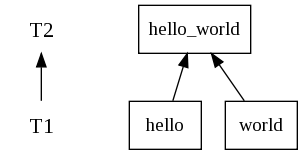
\includegraphics[scale=0.5]{helloworldabstract.png}

The above application is a directed acyclic graph, and it shows three types. Two on tier1 (T1) - hello and world, and one on T2 - hello_world. The T2 hello_world object subscribes to the two T1 objects. The hello_world object simply concatenates the names of the two objects and prints them out.

What will happen when the application starts is that the T1 objects will run concurrently (they do nothing in this simple example), then the T2 object will run. This will read the names of the T1 objects and concatenate them and print the result. The output is below.


\begin{verbatim}
~/src/hello_world$ hello_world
Creating new type hello, type_id: 1
Creating new type world, type_id: 2
Creating new type hello_world, type_id: 3
Loading objects...
Loading hello..
Loading world..
Loading hello_world..
Validating objects...

Num objects on T1: 2
Num objects on T2: 1

Running in single-threaded mode.

Tier 1 running.
Tier 1 ran 2 objects in 6.60419e-05 seconds.

Tier 2 running.
Hello world!
Tier 2 ran 1 objects in 2.88486e-05 seconds.

All tiers ran 3 objects in 0.000231981 seconds.

Exiting after first run as BATCH_MODE is set.
\end{verbatim}

When the application hello_world starts, it first creates the three types we discussed above. Next the objects themselves are loaded. Next the objects are validated and the number of objects on each tier reported. This application is set to use single-threaded mode to keep the output orderly. 

Next we'll see how these types are defined.

\section{The .t4 files}

The way types are defined is in their *.t4 file in the src directory. The types hello and world are the simplest possible as they do absolutely nothing and thus .t4 files are empty, but hello_world.t4 is shown below:

\begin{verbatim}
sub
    hello hello
    world world
\end{verbatim}

The .t4 files are split into three sections. The sub section as shown above describes the type and name of the other trad4 types to which this this type subscribes. In this case hello_world subscribes to two types, the first being a hello object called hello, and the second a world object called world.

The other two sections are static - where the object keeps it's static data which is loaded from the database, and the pub section - where the intermediate and final values of the object's calculate function are stores and published to the world. Neither of these two sections are used in this simple model.

Each type must also have an entry in the object_types.t4s file (the 's' stands for system). This is shown below:

\begin{verbatim}
#type_id, tier, name
1,1,hello
2,1,world
3,2,hello_world
\end{verbatim}


The type_id must be unique. From this we can see type hello has an type_id of 1 and exists on tier 1 and world has an type_id of 2 and also exists on tier 1. The hello_world type has an type_id of 3 and exists on tier 2.

\section{The Calculate Function}

Now we have described the type, we must specify what is does, in this case concatenating the names of the two objects and printing it out.

A stub calculate function is generated for you by trad4, and is found in the objects directory. Again, hello and world do nothing but hello_world's calculate function is shown below:

\begin{verbatim}
int calculate_hello_world( obj_loc_t obj_loc, int id )
{
    cout << object_name(hello_world_hello) << " " << object_name(hello_world_world) << "!" << endl;

    return 1;
}
\end{verbatim}

Trad4 pulls all the information from the sub objects into the scope of this function using macros. You need not concern yourself how these macros work, just think of then as variables which will do what you expect. The functions signature is boilerplate to allow the macros to work and can be ignored. Also ignore the return value for now.

In this case there's very little information in the sub objects, just their id. The macros used above are shown below (from gen/objects/hello_world_macros.h):

\begin{verbatim}
sub:
    id hello_world_hello
    id hello_world_world
\end{verbatim}

So this shows that within calculate_hello_world there's a variable hello_world_hello in scope that will return the id of the hello object. Likewise there's a variable hello_world_world that will return the id of the world object. These id's we can use in the trad4 object_name function to return the name of the object, which is exactly what calculate_hello_world does above.

\chapter{Example: Simple Maths}

\section{Introduction}

We're going to move on to a more complex example in order to demonstrate the concurrency. We want to model the following simple problem:

\begin{math}
  \begin{array}{ l c }
        & z = x + y   \\
        where         \\
        & x = a + b   \\
        & y = c + d   \\
        and           \\
        & a = 7       \\
        & b = 14      \\
        & c = 6       \\
        & b = 27      \\
  \end{array} 
\end{math}

The abstract graph for simple_maths is as follows:

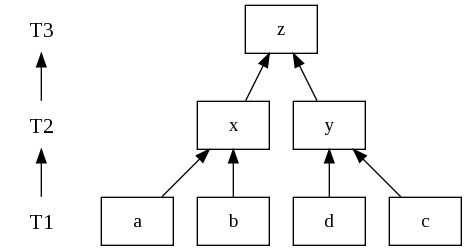
\includegraphics[scale=0.5]{simplemathsabstract.png}

From this we can see that should a, b, c, and d all change we can run x and y at the same time, followed by z. Likewise, if only a changes we only need to recalculate x. Another point to note it that there is just one instance of \begin{math} a + b\end{math} in the whole system - any other object that requires that result subscribe to the x object and read it from there. We will see later how it's possible to decompose quite complex problems into trad4 applications and have fragments of them run concurrently.

\section{The .t4 Files}

In this example the .t4 files are a little more interesting. Below, a.t4:

\begin{verbatim}
static
    int out
\end{verbatim}

Here type a has only one member, it's in the static section and it's an int called out. It's in the static section as the data is stored in the database. More on this below.

The .t4 file for b, c and d are identical to a's and not shown. The .t4 file for x is shown below:

\begin{verbatim}
sub
    a a
    b b

pub 
    int out
\end{verbatim}

Here type x has three members. The first two are in the sub section and shows x subscribes to a type a called a, and a type b of name b. It also has an int called out in the pub section, where the result of \(a + b\) will be stored to be consumed by z.

The .t4 files for y and z are similar to x's and not shown. In fact there's a more concise way to arrange similar t4 types using inheritance of interface (IoI), as discussed in general_computer below.

\section{The Calculate Function}

The calculate functions for a, b, c and d do nothing, as the types consist entirely of a single static member which is just published to to the world at large without any processing. The calculate_x function is shown below:

\begin{verbatim}
int calculate_x( obj_loc_t obj_loc, int id )
{
    x_out = a_out + b_out;

    return 1;
}
\end{verbatim}

Again these variables are provided by macros (from gen/objects/x_macros.h):


\begin{verbatim}
sub:
    id x_a
    int a_out

    id x_b
    int b_out

static:

pub:
    int x_out
\end{verbatim}

Here you can see for each sub member two variables are provided, in a's case these are x_a which provides it's id, and a_out where a will publish it's static data. Also in the pub section is the int x_out, where the result of  \(a + b\) is published. So calculate_x takes the published a_out and b_out variables, adds them and publishes the result in x_out.

The calculate functions for y is very similar to that of x, but z's includes some output:

\begin{verbatim}
int calculate_z( obj_loc_t obj_loc, int id )
{
    z_out = x_out + y_out;

    cout << "z_out: " << z_out << endl;

    return 1;
}
\end{verbatim}

\section{The Data}
\label{sec:The Data}

In the first example hello_world we ignored the database to keep things simple, but we need to introduce it now. Trad4 uses sqlite - a serverless database written in C. All the tables you need (and some of the data) are generated for you by the precompiler, but you need to provide the data for. 

At this stage we also need to distinguish between objects and types. Types are the trad4 types as described in their .t4 files and calculate function. Objects are the running, instantiated types, described in the database. This discussion is confused by the fact that in this application and in hello_world, each type has a single instantiated object with type_id=id. This will become clearer later as we have multiple objects of particular types as in bond_risk below.

The main table in the database is the object table, in which every object has an entry. This table is shown below:
 
\begin{verbatim}
create table object (
    id int, 
    type_id int,
    tier int,
    name char(32),
    log_level int,
    need_reload int
);
\end{verbatim}

The id is the unique id of this object. The type_id gives the type of the object, as described in the object_types.t4s file described above. The tier gives the tier this object exists on, as objects of the same type can exist on different tiers in certain circumstances. The name field holds the name of the object which we pressed into service in hello_world. The log_level controls the level of logging the object does, and need_reload controls whether of not the object needs to be reloaded when the application receives a reload signal (more on this later).

As well as the object table, each type has one or more type-specific tables. In simple_maths this is just one table per type. Below is the table for a (from gen/object/sql):


\begin{verbatim}
create table a (
    id int,
    out int
);
\end{verbatim}

There is the primary key id, plus the static value of the out variable. So the data for object a of type a is given by (from data/worked_example/a.sql):

\begin{verbatim}
insert into object values ( 1, 1, 1, "a", 1, 0 );
insert into a values ( 1, 7 );
\end{verbatim}

So we can see an object with id of 1, type 1 running on tier 1 called "a" with log_level 1 and need_reload set to 0. In type-specific table a there's the primary key id and the value of out, given by 7. The data for objects b, c and d are similar to this, except they have different ids, type_ids, names and static out values as described above. The data for object x is given by:


\begin{verbatim}
insert into object values ( 5, 5, 2, "x", 1, 0 );
insert into x values ( 5, 1, 2 );
\end{verbatim}

This shows an object with id 5, type 5, tier 2 etc. In type-specific table x there's the primary key id and the ids of the two objects to which x subscribes, namely a with id 1 and b with id 2. 

Now we have the full description of this application we can run it:

\begin{verbatim}

~/src/simple_maths$ simple_maths
Creating new type y, type_id: 6
Creating new type c, type_id: 3
Creating new type a, type_id: 1
Creating new type b, type_id: 2
Creating new type x, type_id: 5
Creating new type d, type_id: 4
Creating new type z, type_id: 7
Loading objects...
Loading y..
Loading c..
Loading a..
Loading b..
Loading x..
Loading d..
Loading z..
Validating objects...

Num objects on T1: 4
Num objects on T2: 2
Num objects on T3: 1

Running in single-threaded mode.

Tier 1 running.
calculate_a( a )
calculate_b( b )
calculate_c( c )
calculate_d( d )
Tier 1 ran 4 objects in 8.89301e-05 seconds.

Tier 2 running.
calculate_x( x )
calculate_y( y )
Tier 2 ran 2 objects in 4.60148e-05 seconds.

Tier 3 running.
calculate_z( z )
z_out: 54
Tier 3 ran 1 objects in 3.60012e-05 seconds.

All tiers ran 7 objects in 0.000287056 seconds.

\end{verbatim}

As in the previous example you can see the types being created and the objects being loaded and validated. Then from the report you can see we have 4 objects in T1, 2 on T2 and 1 on T3, as expected. Then the tiers are run as before, with z producing the output 54.

\section{Feeding in change}

In this case the applications doesn't terminate after the first time all the tiers are run, but loops over the objects on T1 looking for change. We introduce change as follows:

\begin{enumerate}

\item Change the required values in the database and set the need_reload flag.
\item Send the application a signal to indicate something has changed.

\end{enumerate}

So we'll update a's static data and trigger a reload. First we log into the database and make the changes:

\begin{verbatim}

~/src/simple_maths$ t4db
sqlite> update a set out=19 where id=1;
sqlite> update object set need_reload=1 where id=1;

\end{verbatim}

And send the reload signal:

\begin{verbatim}

~/src/simple_maths$ send_reload.sh

\end{verbatim}

This produces the following output:

\begin{verbatim}

Tier 1 running.
calculate_a( a )
Tier 1 ran 1 objects in 5.00679e-05 seconds.

Tier 2 running.
calculate_x( x )
Tier 2 ran 1 objects in 3.91006e-05 seconds.

Tier 3 running.
calculate_z( z )
z_out: 66
Tier 3 ran 1 objects in 4.19617e-05 seconds.

\end{verbatim}

Notice only a, x and z fired, the minimum needed to recalculate z given that only a had changed. Next we'll update b and c (ids 2 and 3):

\begin{verbatim}

~/src/simple_maths$ t4db
sqlite> update b set out=23 where id=2;
sqlite> update c set out=46 where id=3;
sqlite> update object set need_reload=1 where id in ( 2, 3 );

\end{verbatim}

This produces the following output:

\begin{verbatim}
Tier 1 running.
calculate_b( b )
calculate_c( c )
Tier 1 ran 2 objects in 7.29561e-05 seconds.

Tier 2 running.
calculate_x( x )
calculate_y( y )
Tier 2 ran 2 objects in 3.60012e-05 seconds.

Tier 3 running.
calculate_z( z )
z_out: 115
Tier 3 ran 1 objects in 2.69413e-05 seconds.
\end{verbatim}

From this you can see both b and c on T1 and x and y on T2 both run concurrently. 

If fact in this example they don't as we're running is single threaded mode to keep the output orderly, but this is easily set with the environment variable NUM_THREADS, e.g.:

\begin{verbatim}
~/src/simple_maths$ export NUM_THREADS=64
~/src/simple_maths$ simple_maths
\end{verbatim}

\chapter{Example: Bond Risk}

\section{Introduction}

Now we're going to examine a real world example of the trad4 architecture from the world of finance - bond_risk. This is a model that calculates the risk on two financial instruments - bonds and outright trades - that depend on the expected future values of interest rates. This is explained in more detail below, but first, the abstract graph:




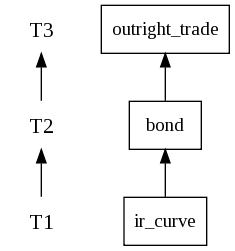
\includegraphics[scale=0.5]{bondriskabstract1.png}

\subsection{T1: ir_curve}

The first type on T1 is ir_curve. This contains information about the expected future value of interest rates. We observe information from the markets to obtain a set of input_rates, and construct a curve starting today and going forward to a set endpoint (say 20 years). This constructed curve has an entry for each day from today to 20 years containing information derived from our input rates, which will be consumed by the T2 bond objects. The key point to note about ir_curves is that they are expensive to construct - the various algorithms used to bootstrap and interpolate the various curves are computationally expensive.

\subsection{T2: bond}

The second type on T2 is bond. A bond is a financial instrument that you buy for a certain price, and pays you fixed payments or coupons at a certain rate until it matures (say 20 years). Because it pays you money at a fixed rate (say 3\% per year), it will become more or less valuable depending on the current and expected future value of interest rates. A bond that pays 3\% when interest rates are 3% will be worth 100 (they are bought and sold in lots of 100), but it will have a higher price when interest rates are at 1\% (say 102.8) then when they are at 5\% (say 97.8) because they pay out more than that same £100 would in the bank (at 3%).

TODO: Real data from worked_example.

\subsection{T3: outright_trade}

The last type on T3 is outright_trade. This trade captures value of the purchase of a bond at a particular time. If you buy a bond with a price of £100 today, and the bond price rises in the future because interest rates fall, the present value (pv) of that trade increases. If you sell the bond at that future time you stand to make a profit. This profit or loss (pnl) is calculated by the original price of the bond and the bond's current published price.

\subsection{Risk: pv01}

In addition to bond's price and outright_trade's pv and pnl, there are other risk measures we can produce for these types, and in this example we're going to focus on is pv01. The pv01 of a bond is the amount the price or present value (pv) will change given a small shift - 1 basis point (bp - 100th of a percent) - in interest rates. If a bond has a high pv01 it's price is likely to be very sensitive to interest rate movements and be inherently more risky. A bond with a low pv01 will be less sensitive to interest rates. 

Likewise an outright_trade on a bond with a high pv01 will itself be sensitive to the volatility of the bond, so it will have an indirect sensitivity to interest rates.

The way pv01 is calculated is that the ir_curve is bumped or perturbed up by 1bp and the bond is priced against that perturbed curve. Then then original ir_curve is bumped down by 1bp and again the bond is priced. The difference between these two prices is the pv01.

From the perspective of the trad4 architecture this is quite easy to achieve: We just have the ir_curve type also produce bootstrapped curves perturbed up and down by 1bp. Then bond can read the bumped and un-bumped forward rates directly from the ir_curve objects. 

That's the bulk of the finance bit over for now. We can now discuss the t4 files.

\section{The t4s files}

The bond_risk application uses some more advanced features of trad4, specifically constants, enums, aliases and structures. These will be introduced in the next section and expanded on in section ~\ref{sec:Language Features}. Additionally ir_curve uses array members, which will be discussed in that section.

The t4s files are the trad4 system files that you supply as you need the relevant features. They described below.

\subsection{constants.t4s}

The constants.t4s file allows you to define your own constants that will be in scope in all calculate functions. Below, bond_risk's constants.t4s file:


\begin{verbatim}
TODAY = 40403            # 13/08/2010
END_DATE = 47708         # 13/08/2030

NUM_FORWARD_DAYS = END_DATE - TODAY

NUM_INPUT_RATES = 10

YEAR_BASIS = 365.25
\end{verbatim}

This describes the start and end dates covered by this model, and the number of forward dates are calculated from that data. Also the number of input_rates is set here, as is the year basis which describes how years are calculated.

\subsection{enums.t4s}

You can define your own enums to use in the t4 files in src/enums.t4s. There's only one enum used in bond_risk, used to indicate the direction of a trade:

\begin{verbatim}
buy_sell_enum
    BUY
    SELL
\end{verbatim}


\subsection{aliases.t4s}

Aliases are simply typedefs, used to clarify your t4 files and structures:

\begin{verbatim}
date = long int
\end{verbatim}

\subsection{structures.t4s}

Any structures you require in your t4 files can be described in structures.t4s. Again there's only one structure used in bond_risk, and that's a rate, described by a value on a particular date (the date given in aliases.t4s):

\begin{verbatim}
rate
    double value
    date asof
\end{verbatim}

Given the above definitions, we can now tackle bond_risk's t4 files. We will look at each type in turn.

\section{ir_curve}

\subsection{The t4 files}

The t4 files are divided into three different sections (all of them optional) - there's the sub section, which lists the other types to which this type subscribes, the static section which is driven by the object's database tables, and the pub section where the results of the calculations using it's static and the pub and static sections of the objects to which it subscribes. These will be discussed in more detail below.

\begin{verbatim}
static
    rate input_rates[NUM_INPUT_RATES]

pub
    double interest_rate_interpol[NUM_FORWARD_DAYS]
    double discount_rate[NUM_FORWARD_DAYS]
    double discount_rate_p01[NUM_FORWARD_DAYS]
    double discount_rate_m01[NUM_FORWARD_DAYS]
\end{verbatim}

\subsubsection{The static section}

The static section is populated from the object's database tables. This data is loaded when the object starts, and may be reloaded at run-time. The static section is published to the rest of the world, but it's not touched by the calculate function.

In this section above we can just see the input_rates, which are an array of rates - the structure defined above - of length NUM_INPUT_RATES as defined in constants.. This is an input to our model, as we're going to move interest rates up and down to see how our bond's and trade's price and risk respond. 

\subsubsection{The pub section}

The pub section is where the results of the object's calculate function are published to the rest of the world. The variables in this section are zeroed when the object starts, and are used as intermediate and final results in the calculate function. If you add a variable to the pub section you will not need to modify the database.

In this section we have four arrays of doubles of length NUM_FORWARD_DAYS. The interest_rate_interpol array is used to store the interpolated input_rates. The other three arrays store the discount_rate - calculated form the interpolated input_rates, and the discount_rate perturbed up and down by one basis point ( _p01 and _m01 respectively). This will be used by other objects to calculate their risk as described below.

\subsection{The calculate function}

\subsubsection{The static section}

This static data is available in the calculate function using the provided macros:

\begin{verbatim}
static:
    rate ir_curve_input_rates[NUM_INPUT_RATES]
    double ir_curve_input_rates_value( NUM_INPUT_RATES )
    date ir_curve_input_rates_asof( NUM_INPUT_RATES )
\end{verbatim}

Given NUM_INPUT_RATES=10, you can use these macros to access the static data in your calculate function as follows:

\begin{verbatim}

    // Get a copy of the first rate
    rate start_rate = ir_curve_input_rates[0];
    // Get a copy of the last rate
    rate end_rate = ir_curve_input_rates[NUM_INPUT_RATES-1];

    // Output the asof date and rate of the start_rate
    cout << "start_rate.asof: " << start_rate.asof << endl;
    cout << "start_rate.value: " << start_rate.value << endl;

    // Loop thought the input rates, outputting the rate and date.
    for ( int i = 0 ; i < NUM_INPUT_RATES ; i++ )
    {
        cout << ir_curve_input_rates_asof( i ) << endl;
        cout << ir_curve_input_rates_value( i ) << endl;
    }

\end{verbatim}

For those financial professionals among you I should make clear that these input_rates contain the bootstrapped forward rates as I've avoided including a bootstrapper to keep things simple. These rates still require interpolation at a daily granularity and conversion into discount factors.

\subsubsection{The pub section}

The pub section is where the results of the object's calculate function are published to the rest of the world. The variables in this section are zeroed when the object starts, and are used as intermediate and final results in the calculate function. If you add a variable to the pub section you will not need to modify the database.  

In this section we have four arrays of doubles of length NUM_FORWARD_DAYS. The interest_rate_interpol array is used to store the interpolated input_rates. The other three arrays store the discount_rate - calculated form the interpolated input_rates, and the discount_rate perturbed up and down by one basis point ( _p01 and _m01 respectively). This will be used by other objects to calculate their risk as described below. 

This pub data can be written to within the calculate function using the provided macros:
\begin{verbatim}
pub:
    double ir_curve_interest_rate_interpol[NUM_FORWARD_DAYS]
    double ir_curve_discount_rate[NUM_FORWARD_DAYS]
    double ir_curve_discount_rate_p01[NUM_FORWARD_DAYS]
    double ir_curve_discount_rate_m01[NUM_FORWARD_DAYS]
\end{verbatim}

Given NUM_FORWARD_DAYS = END_DATE - TODAY, you can use these macros in your calculate function as follows:

\begin{verbatim}
    // Calculate the interpolated rate
    // For details please see bond_risk/objects/ir_curve.c
    ir_curve_interest_rate_interpol[i - TODAY] = ( i*gradient + y_intercept );

    // Calculate the discount factor, plus the two perturbed discount factors
    for ( int i = 0 ; i < NUM_FORWARD_DAYS ; i++ )
    {
        num_years = i / YEAR_BASIS;

        ir_curve_discount_rate[i] = exp( -ir_curve_interest_rate_interpol[i] * num_years );
        ir_curve_discount_rate_p01[i] = exp( -(ir_curve_interest_rate_interpol[i] +0.0001) * num_years );
        ir_curve_discount_rate_m01[i] = exp( -(ir_curve_interest_rate_interpol[i] -0.0001) * num_years );
    }
\end{verbatim}

\section{bond}

\subsection{The t4 files}

\begin{verbatim}
sub
    ir_curve ir_curve

static
    date start_date
    date maturity_date
    int coupons_per_year
    double coupon

pub
    double price
    double pv01
\end{verbatim}

\subsubsection{The sub section}

In the sub section, we can see that bond subscribes to an ir_curve.

\subsubsection{The static section}

In the static section we can see the static data that makes up a simple bond. They have a start_date, the date the bond was issued and is some time in the past. They have a maturity_date when the bond matures - ceases paying out and pays back the 100 you could have bought for at par. The coupons_per_year member describes how often the bond pays, so coupons_per_year=1 pays out once a year and coupons_per_year=4 pays out every quarter. Lastly there's the coupon, which is the rate at which it pays each coupon (e.g. 3% pa).

\subsubsection{The pub section}

The pub section is where the results of bond's calculate function are stored and published. There is the bond's price, calculated form the bond's static and ir_curve's pub section, and pv01 which uses the _p01 and _m01 sections of ir_curve.

\subsection{The calculate function}

\subsubsection{The sub section}

The sub macros available in bond's calculate function pull all the pub and static sections of ir_curve into the scope of the function (from gen/objects/bond_macros.h):

\begin{verbatim}
sub:
    id bond_ir_curve
    rate ir_curve_input_rates[NUM_INPUT_RATES]
    double ir_curve_input_rates_value( NUM_INPUT_RATES )
    date ir_curve_input_rates_asof( NUM_INPUT_RATES )
    double ir_curve_interest_rate_interpol[NUM_FORWARD_DAYS]
    double ir_curve_discount_rate[NUM_FORWARD_DAYS]
    double ir_curve_discount_rate_p01[NUM_FORWARD_DAYS]
    double ir_curve_discount_rate_m01[NUM_FORWARD_DAYS]
\end{verbatim}

We can use these in the calculate function as follows:


\begin{verbatim}















\end{verbatim}

\subsubsection{The static section}

\subsubsection{The pub section}

\section{outright_trade}



\section{The Concrete Graph}

In Section ~\ref{sec:The Data} the distinction between types and objects was made. This becomes clearer now as in this data set we will have two ir_curves, five bonds and nine outright_trades. These objects - instantiated types - are shown on the concrete graph represented by ovals containing the object name. This is shown below:

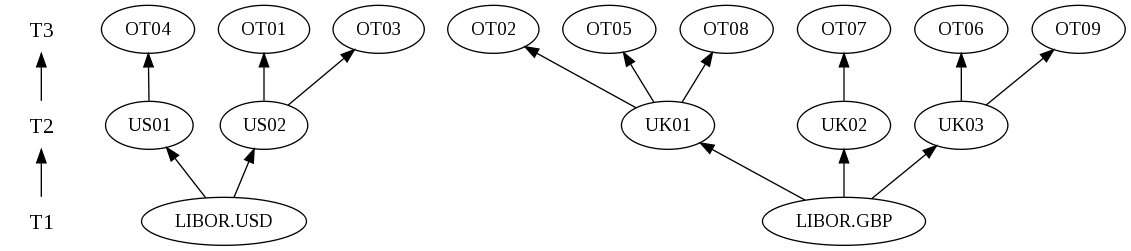
\includegraphics[scale=0.3]{bondriskconcretesmallset.png}

From this we can see the two ir_curves in two different currencies LIBOR.USD and LIBOR.GBP on T1. Then we can see the five bonds on T2, two of which were issued in USD (US01 and US02) which subscribe to LIBOR.USD, and three of which were issued in GBP which subscribe to LIBOR.GBP. Lastly we have the nine outright_trades (OT01 etc.) which subscribe to various bonds.









\chapter{New Application Walk-through}

\section{Run create_new_app.sh}

Change directory into trad4's bin directory and run the script, giving your new app name as the argument.

\begin{verbatim}
    trad4/bin$ ./create_new_app.sh <app_name>
\end{verbatim}

This will create the directory structure for your new application, plus a couple of files you'll be needing.

For the rest of this chapter substitute simple_maths for your application, or follow along with a downloaded  distribution of simple_maths.

\section{Source your .conf file}

You should always source the relevant .conf file at the beginning of each session to set the environment  up:

\begin{verbatim}
simple_maths$ . ./simple_maths.conf
\end{verbatim}

\section{Write your .t4 files}

Set out the sub, static and pub sections. For example, the .t4 file for the type 'a' from simple_maths is:

\begin{verbatim}
static
    int out
\end{verbatim}

As you can see, this type just has a single static variable of type int. This is loaded when the object is started and doesn't change unless it reloads a new value from the database.

The .t4 file for the type 'x' from simple_maths is:

\begin{verbatim}
sub
    a a
    b b

pub 
    int out
\end{verbatim}

Type x has a sub section, describing the type and name of the objects to which it subscribes. In this case it's a type a as described above and a type b (not shown, but identical to a.t4). There is one variable in the pub section this is where x publishes it's output value, called 'out' of type int.

The sub types in the .t4 files must always be of another trad4 type. The static and pub types can be of the following built-in C++ types:

\begin{itemize}
\item int
\item char
\item float
\item double
\item long
\end{itemize}

Arrays are supported in the sub, static and pub sections. Also, constants, enums, aliases and structures can be defined and also used in the static and pub sections. More on this later.

\section{Edit your object_types.t4s file}

This file contains an entry for each type:
\begin{verbatim}
#type_id, tier, name
1,1,a
2,1,b
3,1,c
4,1,b
5,2,x
6,2,y
7,3,z
\end{verbatim}

Each type must have it's own unique type_id, it's tier must be specified and it's name must be unique. 
Anything to the right of a hash will be considered a comment and ignored.

In this case there are seven types. The T1 types are a,b,c and d. There are two T2 types x and y, and one T3 type z.

\section{Run the trad4 precompiler}

The precompiler ­ precomp.pl ­ is aliased to 't4p':

\begin{verbatim}
    $ t4p
\end{verbatim}

This will create several files under your root directory, the most important of which to you are the files under simple_maths/objects. These files ­ one per object ­ contain the stub calculate functions that you must provide the logic for.  You could supply this functionality now, or if you're impatient you can skip to the next step and supply the functionality later.

A generated file you will be needing are the macros under simple_maths/gen/objects and have the file name $<$type$>$_macro.h. There's a comment at the top of this file that shows you what's in scope for the calculate function.

Also generated by the precompiler are the .table files that specify the default database structure. These are found under simple_maths/gen/sql. There is even some dummy data created under simple_maths/data/dummy_data.

The rest of the files produced by the precompiler provide the guts of the trad4 application and you will probably not be interested in. They reside with the macros under simple_maths/gen/objects.

The precompiler supports various command­line options, e.g.:

\begin{verbatim}
simple_maths]$ t4p -h
Usage: precomp.pl [OPTION]
The trad4 precompiler.

  -o <object>    precompile <object> only
  -k             continue on error
  -c             remove all generated files
  -a             remove all generated files and regenerate
  -v             verbose - dumps internal structures
  -d             generate documentation
  -h             display this help and exit
\end{verbatim}

\section{Choose how many threads you need}

To set the number of threads used you set the NUM_THREADS environment variable.

\begin{verbatim}
    $ export NUM_THREADS=16
\end{verbatim}

The default for a new application is 0, which means the master thread does all the work. Setting NUM_THREADS=1 means there is one master thread and one worker thread. The maximum is 4096.

As with all the environment variables, they can be set in app.conf file.


\section{Create the database}

Trad4 uses sqlite, a server-less flat file database. The structure is generated for you by the precompiler, as is some dummy data to get you started.

\begin{verbatim}
    $ recreate_db.sh
\end{verbatim}

This will load the table definitions generated under simple_maths/gen/sql into the DB, and (re)create the 
system tables.

Next, load the default data set:

\begin{verbatim}
    simple_maths/data$ reload_db.sh default_set/
\end{verbatim}

\section{Compile the application}

To compile the application, just type make:

\begin{verbatim}
    simple_maths$ make
\end{verbatim}

This will compile and link your application and produce an executable binary of the same name as your 
application. You can run it now if you like. 

\begin{verbatim}
    simple_maths$ bin/simple_maths
\end{verbatim}

You should see the types being created, then the load functions being called and the objects being created (there's a one-to-one correspondence between the types and objects in this simple model). The objects are then validated and a short report is produced. The tiers are then run in turn and all the calculate functions being called, but they won't do anything yet as the logic hasn't yet been provided.

The application should then exit as BATCH_MODE is set as default, which caused the application to exit after the first run.

\section{The Calculate Function}

\section{The Object Data}

\section{Triggering an update}

To trigger an update you first need to set the need_reload flag on the object table to 1 for those objects you want to reload:

\begin{verbatim}
    SQL> update object set need_reload = 1 where id in (...);
\end{verbatim}

You'll then need to unset BATCH_MODE so that the application continues running. Then you send a signal to your application that there's one or more objects that need to be reloaded:

\begin{verbatim}
    $ send_reload.sh 
\end{verbatim}

You will then see all the objects triggering in the order you expect. All the calculate functions will be called, and you should see the affect of your update on the output.

Note that the dummy_data set created for you has need_reload=1 for all objects.

\section{Tips and Tricks}

Keep it simple for now and restrict yourself to two or three types when you're starting a new application.

\chapter{Language Features}
\label{sec:Language Features}

\chapter{Tips and tricks}

\chapter{Living with trad4}

\chapter{Hardware considerations}

\appendix

\chapter{How trad4 works}

\end{document}

